\begin{figure}[tbp]
  \centering
  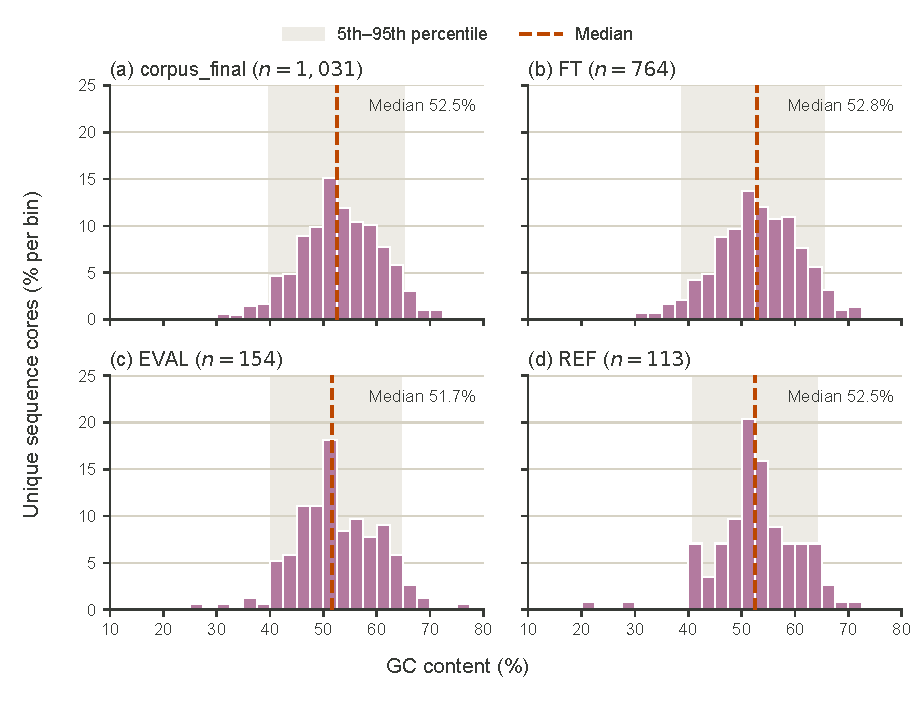
\includegraphics[width=\textwidth]{figures/final_corpus_gc_distribution.pdf}
  \caption[GC-content distributions for the final corpus and its partitions.]{%
  GC-content distributions for (a) the complete final corpus, (b) FT, (c)
  EVAL, and (d) REF. Histograms show the relative frequency of unique sequence
  cores, so a core associated with multiple targets is counted once within
  each panel. The complete corpus contains 1,031 unique sequence cores,
  partitioned without overlap into FT ($n=764$), EVAL ($n=154$), and REF
  ($n=113$), which reconcile to the corpus total. Dashed lines mark the panel
  medians (52.5\%, 52.8\%, 51.7\%, and 52.5\%, respectively), and shaded
  regions mark the corresponding 5th--95th percentile intervals. GC content
  was not an explicit split-balancing objective; the similar profiles
  therefore provide an independent check that partitioning did not materially
  distort the corpus composition.}
  \label{fig:final-corpus-gc-distribution}
\end{figure}
